\documentclass[useAMS,usenatbib]{mn2e}
\usepackage{footnote,graphicx,natbib,color,multirow,amsmath,url,amssymb,tabularx,hyperref,amssymb, mathtools, listings, float}
\usepackage{aas_macros}

\hypersetup{
    colorlinks,
    citecolor=blue,
    filecolor=black,
    linkcolor=black,
    urlcolor=black
}

\def\lesssim{\mathrel{\hbox{\rlap{\hbox{\lower3pt\hbox{$\sim$}}}\hbox{\raise2pt\hbox{$<$}}}}}


\begin{document}

\title[SFH gradients in MaNGA AGN]{MaNGA: Quenching gradients of AGN host galaxies}
\author[Smethurst et al. 2017]{R. ~J. ~Smethurst,$^{1}$ et al.
\\ $^1$ Oxford Astrophysics, Department of Physics, University of Oxford, Denys Wilkinson Building, Keble Road, Oxford, OX1 3RH, UK
}

\maketitle

\begin{abstract}
\end{abstract}

\begin{keywords}
galaxies -- photometry, galaxies -- statistics, galaxies -- morphology
\end{keywords}

\section{Introduction}\label{sec:intro}
One of the biggest challenges to $\Lambda$-CDM is the persistent lack of statistically supported evidence of negative AGN feedback occurring across the galaxy population. There are strong theoretical predictions for AGN feedback occurring across the entire galaxy population \citep{Fabian12, Gaibler12}. For example, without AGN feedback to regulate star formation, simulated galaxies grow to unrealistic stellar masses \citep[e.g.][]{silk12}. However, direct observational evidence for quenching caused by AGN across the galaxy population has been elusive. This is in part due to the fact that multiple quenching mechanisms can have similar effects on the observable properties of a galaxy. 

\citet{smethurst16} used optical and NUV global colours to infer the star formation histories of $1,244$ Type 2 AGN. They found that the majority of the AGN had undergone a recent, rapid decline in star formation, not detected in a mass matched control sample of inactive galaxies. This result was promising, suggesting that AGN feedback may be the cause, since AGN have short duty cycles of $\lesssim0.3$~Gyr \citep{martini04} and in simulations are found to cause rapid quenching \citep{tortora09}. However, using the global colours, it was not possible for \citeauthor{smethurst16} to determine whether AGN feedback was the internal cause of the inferred quenching or whether the AGN was merely a consequence of another quenching mechanism (e.g. its activity has been triggered by a galaxy interaction or merger).

The current barrier to our comprehension of the role of AGN feedback in galaxy evolution is understanding the complex interplay of mechanisms controlling this shutdown (or `quenching') of star formation. Multiple quenching mechanisms can have similar effects on the observable properties of a galaxy and it is therefore difficult to pinpoint the effects of one specific mechanism, such as AGN feedback \cite{smethurst17}. The advent of large IFU galaxy surveys make tackling such a problem possible. In this work we utilise data from the MaNGA (Mapping Nearby Galaxies at Apache Point Observatory; \citealt{Bundy15}) survey, which when complete, will provide a spectrum at 127 individual points (`spaxels') in each of the 10,000 galaxies targeted. Such data allows for spatially resolved quenching histories of galaxies to be determined. This combined with carefully controlling the main and control sample selection allows the effects of individual mechanisms to be isolated. 

In this paper we have selected a sample of AGN using multi-wavelength selection methods, along with a mass, visual and kinematic morphology matched control sample. We have derived azimuthally averaged star formation histories for each galaxy using spectral information and the inference code \textsc{snitch} \cite{smethurst19a}. In Section~\ref{sec:data} we describe the MaNGA data used, in Section~\ref{sec:method} we summarise the methods used, in Section~\ref{sec:results} we present our results along with a discussion in Section~\ref{sec:disc}. Finally, we summarise our findings in Section~\ref{sec:conc}. Where necessary we adopt the Planck 2015 \citep{planck16} cosmological parameters with $(\Omega_m, \Omega_{\lambda}, h) = (0.31, 0.69e, 0.68)$. 

\section{Data}\label{sec:data}

\begin{figure*}
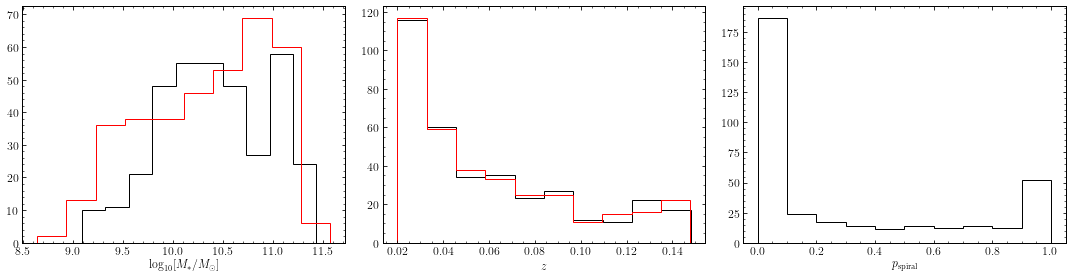
\includegraphics[width=0.9\textwidth]{../data/ellison/figures/control_manga_agn_properties_compare.png}
\caption{Properties of the AGN sample (black) compared with the matched control sample (red). Shown are the stellar mass (left), redshift (middle) and spiral morphology classification from Galaxy Zoo (right; see Section ?). The Anderson-Darling p-values are also shown in each panel.}
\end{figure*}

%Figure 2 is an example SDSS cut out with Halpha, Dn4000 maps etc
% this actually needs to be cut out, halpha, dn4000, hbeta, mgfe, hdeltaA - i.e. the ones I actually use in SNITCH
\begin{figure*}
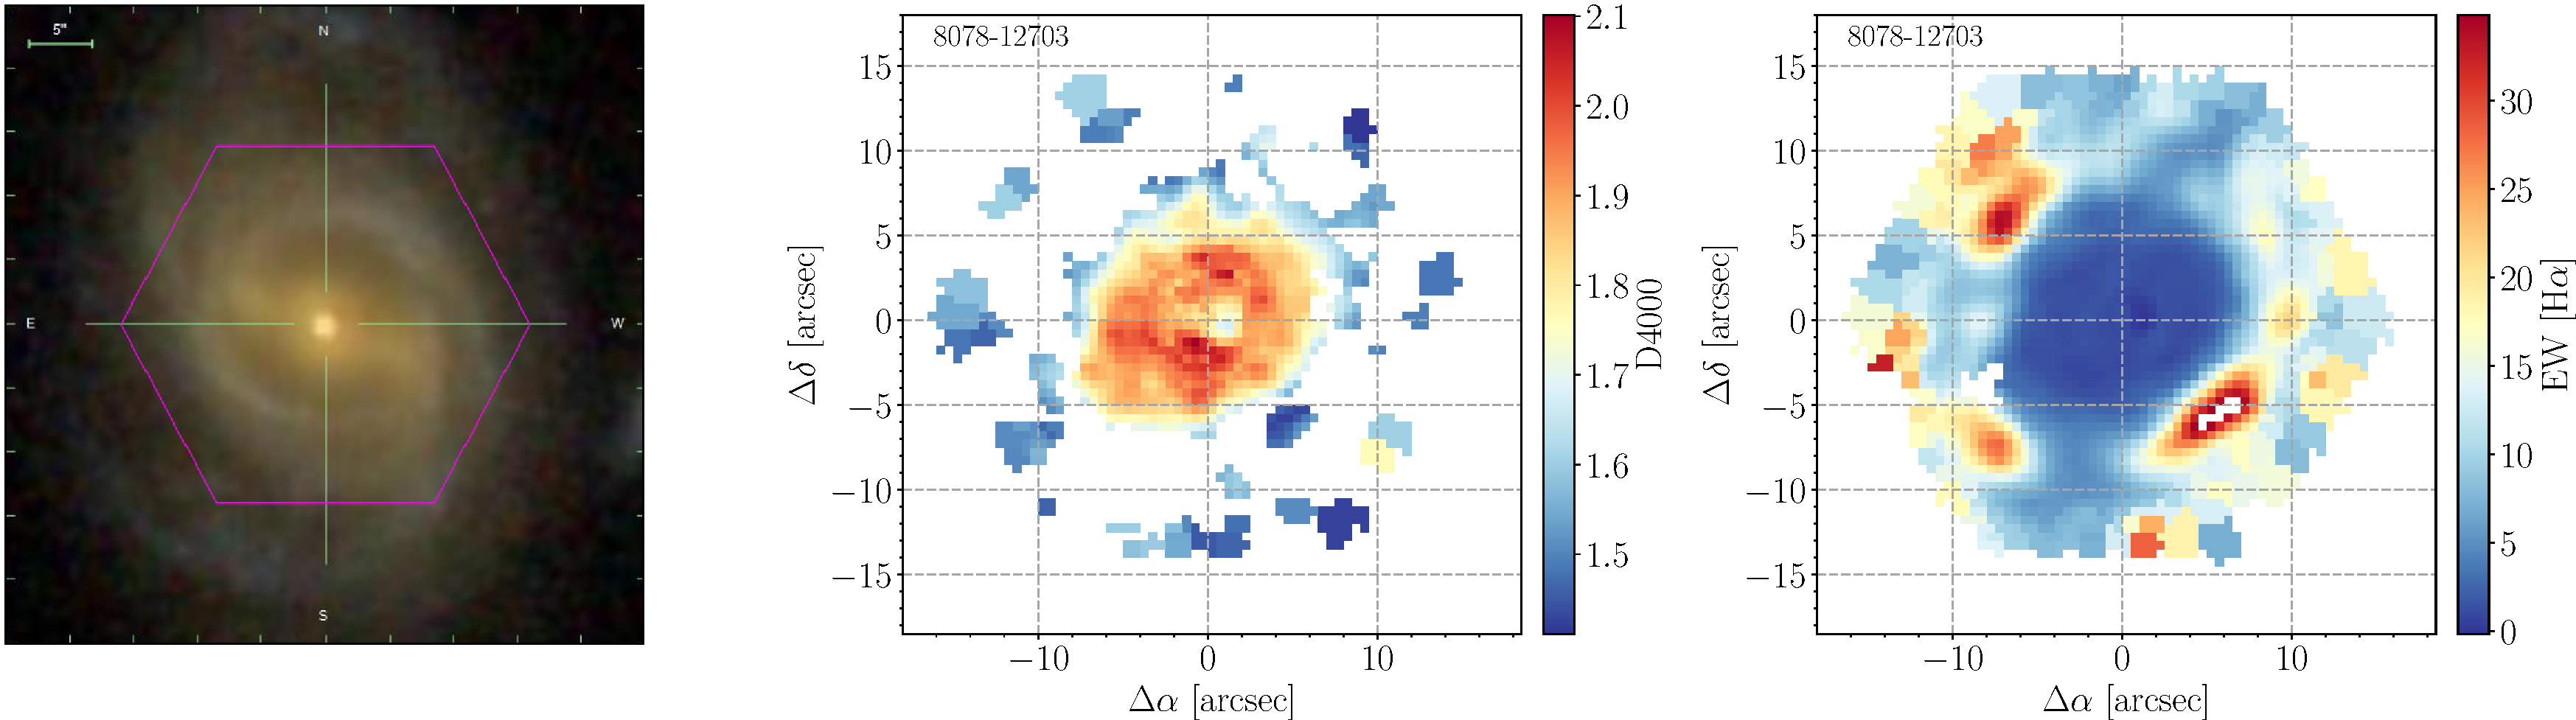
\includegraphics[width=0.9\textwidth]{../data/ellison/figures/image_halpha_vel_map_8078-12703_gal_aligned_ifu_bundles-MAPS-VOR10-GAU-MILESHC.pdf}
\caption{Example SDSS cut out (left) showing the MaNGA fibre foot print (pink hexagon) for MaNGA galaxy 8078-12703. Also shown are  the D4000 (middle) and equivalent width of H$\alpha$ (right) measured from the observed spectra by the MaNGA DAP pipeline. }
\end{figure*}

\begin{figure}
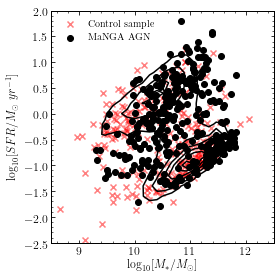
\includegraphics[width=0.45\textwidth]{../data/ellison/figures/manga_agn_SFS_plane.png}
\caption{The stellar mass-star formation rate plane, showing the MaNGA AGN (black circles) and the control sample (red crosses). Also shown in black contours for comparison is the MPA-JHU sample, which clearly show the split in the galaxy population into the star forming sequence (top left) and quenched population (bottom right).}
\end{figure}

\begin{figure}
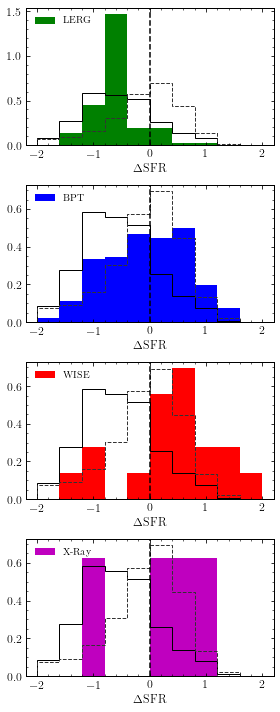
\includegraphics[height=0.75\textheight]{../data/ellison/figures/manga_agn_recreate_ellison.png}
\caption{This figure is a recreation of Figure 3 in Ellison et al. (2016). We show the distribution of the difference in the star formation rate, $\Delta~SFR$ from the expected SFR a galaxy would have if it was on the star forming main sequence of Peng et al. (2010), given a galaxy's mass and redshift. In each panel we show the $\Delta~SFR$ for the control sample (solid line) and the MPA-JHU catalog (dashed line). We have split the AGN sample by the type of AGN, LERGs (top panel, green), optical AGN identified using the BPT diagram (second panel, blue), infrared AGN from WISE (third panel, red), and X-ray AGN from Edelson \& Malkan (2012; 2MASS \& ROSAT) shown in the bottom panel in magenta. For more information on AGN selection see Section ?. This figure confirms the results of Ellison et all, showing how AGN identified at different wavelengths may be at different stages of their evolutionary (and therefore quenching) histories.}
\end{figure}

\begin{figure*}
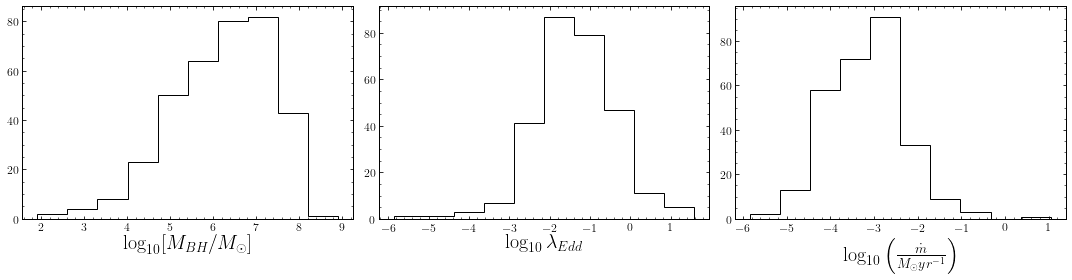
\includegraphics[width=0.9\textwidth]{../data/ellison/figures/mangaagn_sample_agn_properties.png}
\caption{Properties of the MaNGA AGN sample. Shown are the mass of the central supermassive black hole (left; calculated using the method of..., see Section ?), the Eddington ratio (middle) and the accretion rate (right; assuming a radiative efficiency factor $\eta=0.15$, Elvis et al. 2002).}
\end{figure*}


\section{Method}\label{sec:method}

\section{Results}\label{sec:results}


\begin{figure*}
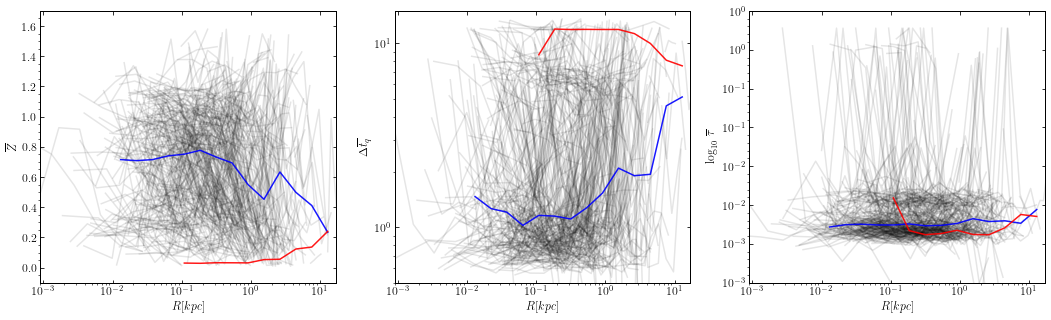
\includegraphics[width=0.9\textwidth]{../data/ellison/figures/manga_agn_spaghetti.png}
\caption{The spatially resolved SFHs with galaxy radius as inferred by \textsc{snitch} for the MaNGA AGN sample. Each MaNGA AGN is shown by a black line for the metallicity (left), time since quenching started (middle) and rate of quenching (right). We also show the median value for bins in the radius for the MaNGA AGN (blue line) and the control sample (red). This figure shows how the quenching histories of current AGN and the control sample are indeed different, in particular, the AGN have quenched more recently than the control sample.}
\end{figure*}

\begin{figure*}
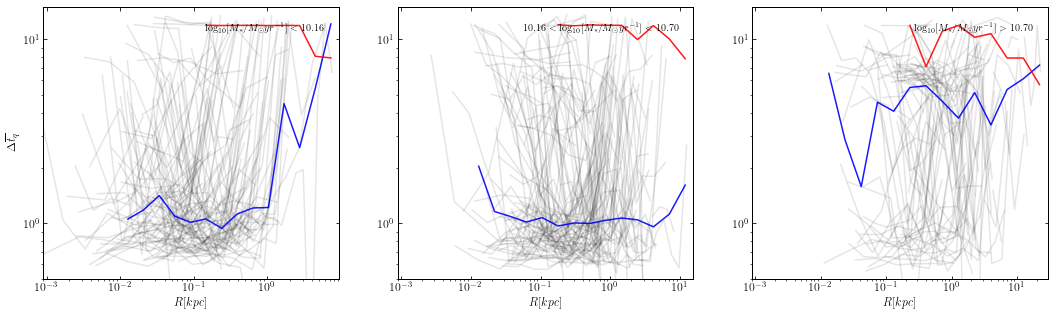
\includegraphics[width=0.9\textwidth]{../data/ellison/figures/median_deltatq_with_kpc_radius_ellison_splitmass.png}
\caption{The spatially resolved time since quenching started against galaxy radius as inferred by \textsc{snitch} for the MaNGA AGN sample, split into low (left), medium (middle) and high (right) stellar mass. These boundaries were chosen to give an equal number of MaNGA AGN in each of the three stellar mass bins. Each MaNGA AGN is shown by a black line. We also show the median value for bins in the radius for the MaNGA AGN (blue line) and the control sample (red) split by stellar mass. This figure shows how lower mass AGN have quenched more recently than high mass AGN, perhaps suggesting that AGN in high mass galaxies have less affect on their host galaxy, supporting results from Smethurst et al. (2016).}
\end{figure*}

\begin{figure*}
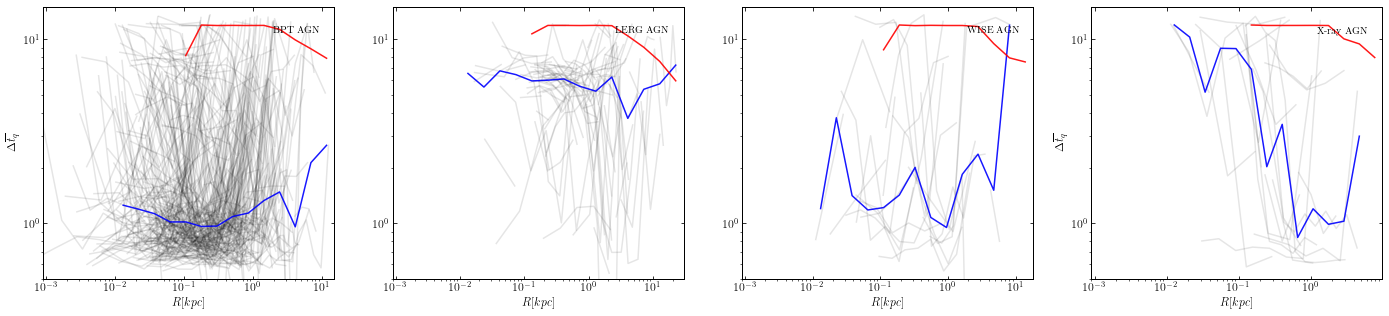
\includegraphics[width=0.9\textwidth]{../data/ellison/figures/median_deltatq_with_kpc_radius_ellison_splitagntype.png}
\caption{The spatially resolved time since quenching started against galaxy radius as inferred by \textsc{snitch} for the MaNGA AGN sample, split by AGN type into optically selected BPT AGN (left), LERGs (second left), infrared WISE AGN (second right), X-RAY AGN (right). Each MaNGA AGN is shown by a black line. We also show the median value for bins in the radius for the MaNGA AGN (blue line) and the entire control sample (red). This figure shows how optical and infrared AGN have quenched more recently than LERGs or X-ray AGN, again supporting the findings of Elison et al. (2012) that multi-wavelength AGN are at different stages of their duty cycles.}
\end{figure*}

\begin{figure*}
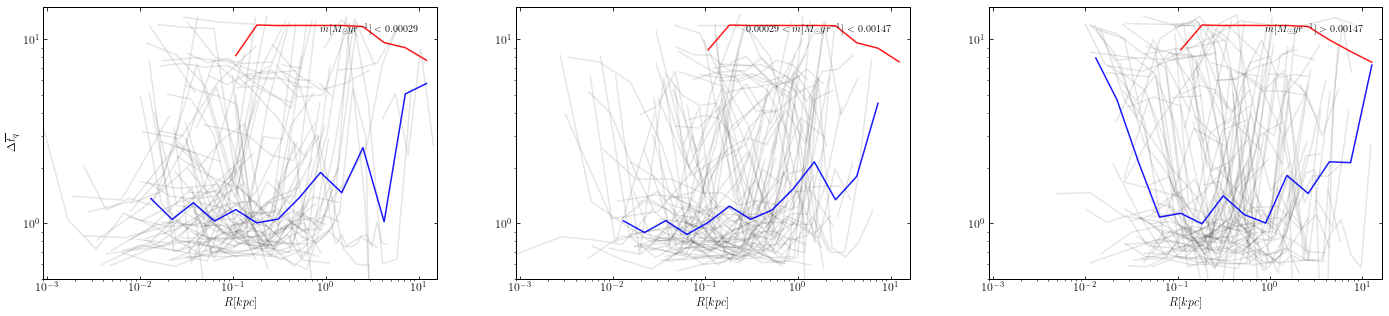
\includegraphics[width=0.9\textwidth]{../data/ellison/figures/median_deltatq_with_kpc_radius_ellison_splitmdot.png}
\caption{The spatially resolved time since quenching started against galaxy radius as inferred by \textsc{snitch} for the MaNGA AGN sample, split into low (left), medium (middle) and high (right) black hole accretion rate. These boundaries were chosen to give an equal number of MaNGA AGN in each of the three accretion rate bins. Each MaNGA AGN is shown by a black line. We also show the median value for bins in the radius for the MaNGA AGN (blue line) and the entire control sample (red). This figure shows how higher accretion rate AGN may have had more effect on their host galaxies in the past.}
\end{figure*}


\section{Discussion}\label{sec:disc}

\section{Conclusions}\label{sec:conc}

\bibliographystyle{mn2e}
\bibliography{refs}  

\end{document}
